\section{Model}\label{sec:model}

The model describes how a given sovereign shock propagates through financial claims. Exposures are in place at date 1. At date 2, sovereign repayments are specified by the scenario and banks settle their debts jointly. The analysis takes these exposures and repayment resources as given; it does not require a model of how firms and households chose their positions. An optional household-saving completion is provided in Appendix~\ref{app:household-completion}.

\subsection{Exposures and sovereign shocks}

There are $C$ countries, collected in $\mathcal C$. Country indices are $c$ or $g$; indices $i,j$ identify network nodes and are restricted to banks where indicated. Each country has households $H_c$, firms $F_c$, banks $B_c$, nonbank financial institutions (NBFIs) $N_c$ and a government $G_c$. Each bank node is a national block; claims within it represent lending among distinct institutions. The network also includes the Eurosystem $E$ and Other counterparties $R$. Write $\mathcal N$ for all nodes and $\mathcal B$, $\mathcal M$ and $\mathcal G$ for banks, NBFIs and governments. The Other counterparties node groups foreign and unclassified positions whose repayments are taken as given.

A claim $x_{ij}\geq0$ runs from creditor $i$ to debtor $j$: rows of the exposure matrix are creditors and columns are debtors. Bank debt $D_i>0$ denotes the liabilities sharing a common repayment rate. Obligations settled at fixed amounts outside this pool are called fixed settlements; they are deducted from both liabilities and repayment resources. The matrix covers selected instruments; its reconciliation with complete balance sheets supplies the remaining net resources. These accounting details are set out in Appendix~\ref{app:calibration-details}.

A sovereign state $s$ specifies default indicators $\delta_c^G(s)\in\{0,1\}$ for each country $c\in\mathcal C$. There are therefore $2^C$ possible sovereign states. Let $\overline r_c^G$ be government $c$'s contractual gross payment per unit of debt securities and $\underline r_c^G$ its payment following default. Its realized payment is
\[
 R_c^G(s)=\begin{cases}
 \overline r_c^G,&\delta_c^G(s)=0,\\
 \underline r_c^G,&\delta_c^G(s)=1,
 \end{cases}
 \qquad 0\leq\underline r_c^G<\overline r_c^G.
\]
These repayments are exogenous: banking outcomes do not change sovereign default or recovery. The scenario also specifies impairments on bank-held firm and household loans. Private borrowing and credit supply remain fixed during clearing.

Other counterparties and the Eurosystem repay at the safe gross rate, normalized to one. They bear losses on their assets without passing them back through their own debt payments. NBFIs also repay in full in the calibration.\footnote{The calibrated buffers imply full NBFI repayment even when their repayments are determined endogenously. Under national pooling and with other net resources fixed, these buffers cover all debt even if the selected claims on banks, other NBFIs and sovereigns pay nothing. Full repayment therefore holds in every equilibrium; Appendix~\ref{app:calibration-details} gives the bound.} Nonbank receipts are therefore fixed within each sovereign state in the reported exercises.

\subsection{Bank resources, distress and repayment}\label{sec:model_banks}

Normalize contractual bank repayment to one. For each bank block $i\in\mathcal B$, $R_i\in[0,1]$ is both the amount paid per unit borrowed and the creditor recovery rate; a claim of size $x_{ji}$ pays $x_{ji}R_i$. Collect these rates in the vector $\mathbf{R}=(R_j)_{j\in\mathcal B}\in\mathcal K$, where $\mathcal K=[0,1]^{|\mathcal B|}$.

Let $a_i(s)\geq0$ collect nonbank receipts net of fixed settlements and the scenario's losses. Bank $i$'s resources before its own default cost are
\[
 A_i(s,\mathbf{R})=a_i(s)+\sum_{j\in\mathcal B}x_{ij}R_j.
\]
We suppress the arguments $(s,\mathbf{R})$ when they are clear from context.

Let $E_i$ denote accounting equity in the reference balance sheet, whose repayment resources are $D_i+E_i$. Define the change in resources relative to this benchmark by
\[
 L_i=D_i+E_i-A_i,
 \qquad A_i-D_i=E_i-L_i.
\]
Thus $L_i>0$ measures the reduction in resources before the bank's own default cost; $L_i<0$ represents a gain relative to the benchmark. We refer to positive $L_i$ as pre-cost losses. These losses first reduce equity and need not entail losses for creditors. The quantity $E_i-L_i$ is remaining pre-cost equity when positive and an accounting shortfall when negative.

Loss headroom $0\leq H_i\leq E_i$ specifies how much of this reduction can occur before the distress threshold is breached. A breach occurs when $L_i>H_i$, equivalently $A_i<D_i+E_i-H_i$. Headroom sets the trigger; all accounting equity remains available to absorb losses. In particular, when $H_i<L_i<E_i$, the threshold is breached even though pre-cost equity remains positive.

A distress episode destroys the fraction $1-\lambda_i^B$ of the remaining estate, where $0<\lambda_i^B\leq1$. This wedge captures franchise disruption and difficult asset realization. It is a cost parameter, not a creditor recovery rate. Partial repayment requires both a headroom breach and a creditor shortfall after this cost:
\begin{equation}
 R_i=\begin{cases}
 \lambda_i^B A_i/D_i,&L_i>H_i\ \text{and}\ \lambda_i^B A_i<D_i,\\
 1,&\text{otherwise}.
 \end{cases}
 \label{eq:bank_repayment}
\end{equation}
Figure~\ref{fig:equity-headroom} illustrates three cases. Within headroom, the bank repays in full. After a breach, repayment remains full if pre-cost equity covers the hypothetical distress cost, $E_i-L_i\geq(1-\lambda_i^B)A_i$, equivalently $\lambda_i^B A_i\geq D_i$. Otherwise, the cost leaves insufficient resources to repay creditors in full. This can occur even with positive pre-cost equity. Figure~\ref{fig:bank-repayment-rule} summarizes the two tests. The rule is a reduced-form description of disorderly distress; a prudential breach is not an automatic legal default.

\begin{figure}[htbp]
\centering
\floatcaption{Headroom, equity and creditor losses: three balance sheets}{Illustrative balance sheets with the same debt, initial equity, headroom and cost parameter. The vertical arrow measures the resource threshold $D_i+E_i-H_i$ from the common zero baseline to the dashed line. Resources below this line breach headroom. Orange indicates the hypothetical distress cost; the solid line below it marks $\lambda_i^B A_i$. In (b), remaining equity covers this cost, so the model specifies full repayment. In (c), the cost exceeds remaining equity and creditors incur losses even though pre-cost equity is positive. The cost is applied only when both conditions in equation~\eqref{eq:bank_repayment} hold.}
\label{fig:equity-headroom}

\resizebox{0.98\textwidth}{!}{%
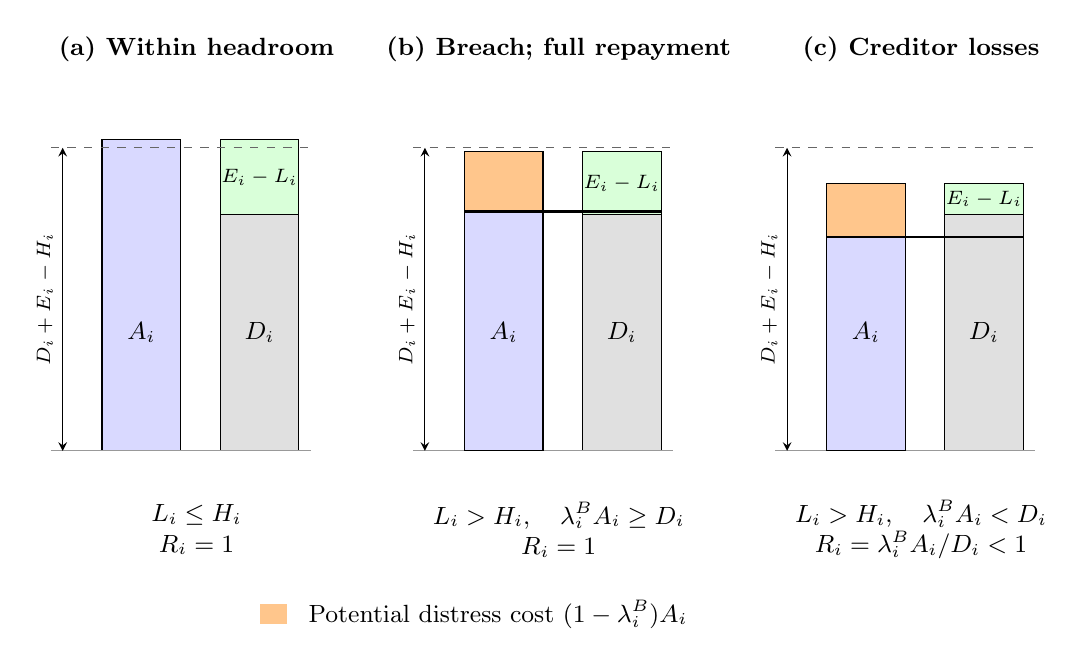
\begin{tikzpicture}[x=1cm,y=1cm,>=stealth,font=\small]
% Common illustrative values: D=3, E=1, H=.15, lambda=.8.
\foreach \shift/\height/\title in {0/3.95/{(a) Within headroom},4.6/3.8/{(b) Breach; full repayment},9.2/3.4/{(c) Creditor losses}} {
 \begin{scope}[xshift=\shift cm]
  \node[font=\small\bfseries,align=center] at (1.2,5.1) {\title};
  \fill[blue!15] (0,0) rectangle (1,\height);
  \draw (0,0) rectangle (1,\height);
  \fill[black!12] (1.5,0) rectangle (2.5,3);
  \fill[green!15] (1.5,3) rectangle (2.5,\height);
  \draw (1.5,0) rectangle (2.5,\height);
  \draw (1.5,3) -- (2.5,3);
  \node at (.5,1.5) {$A_i$};
  \node at (2,1.5) {$D_i$};
  \node[font=\scriptsize] at (2,{(3+\height)/2}) {$E_i-L_i$};
  \draw[black!40] (-.65,0) -- (2.65,0);
  \draw[dashed,black!60] (-.65,3.85) -- (2.65,3.85);
  \draw[<->] (-.5,0) -- node[midway,above,sloped,font=\scriptsize] {$D_i+E_i-H_i$} (-.5,3.85);
 \end{scope}
}
\foreach \shift/\height in {4.6/3.8,9.2/3.4} {
 \begin{scope}[xshift=\shift cm]
  \fill[orange!45] (0,{.8*\height}) rectangle (1,\height);
  \draw (0,0) rectangle (1,\height);
  \draw[thick] (0,{.8*\height}) -- (2.5,{.8*\height});
 \end{scope}
}
\node[align=center] at (1.2,-1) {$L_i\leq H_i$\\$R_i=1$};
\node[align=center] at (5.8,-1) {$L_i>H_i,\quad\lambda_i^B A_i\geq D_i$\\$R_i=1$};
\node[align=center] at (10.4,-1) {$L_i>H_i,\quad\lambda_i^B A_i<D_i$\\$R_i=\lambda_i^B A_i/D_i<1$};
\fill[orange!45] (2,-2.2) rectangle (2.35,-1.95);
\node[anchor=west,font=\small] at (2.5,-2.075) {Potential distress cost $(1-\lambda_i^B)A_i$};
\end{tikzpicture}%
}

\end{figure}


The equivalent resource cutoff is
\[
 T_i=\min\{D_i+E_i-H_i,D_i/\lambda_i^B\}.
\]
Partial repayment occurs when $A_i<T_i$; equality gives full repayment. Because $T_i\leq D_i/\lambda_i^B$, repayment increases on the default branch and can only jump upward at the cutoff. Setting $H_i=E_i$ recovers an accounting-insolvency trigger.

\begin{figure}[htbp]
\centering
\floatcaption{Two conditions for partial bank repayment}{$A_i$ is the pre-cost repayment estate, $D_i$ clearing debt, and $L_i=D_i+E_i-A_i$ the reduction in resources relative to the reference balance sheet. The diagram represents the logical conditions in equation~\eqref{eq:bank_repayment}; settlement is simultaneous. The second test uses resources after the hypothetical cost to determine whether a credit event entails a creditor shortfall.}
\label{fig:bank-repayment-rule}

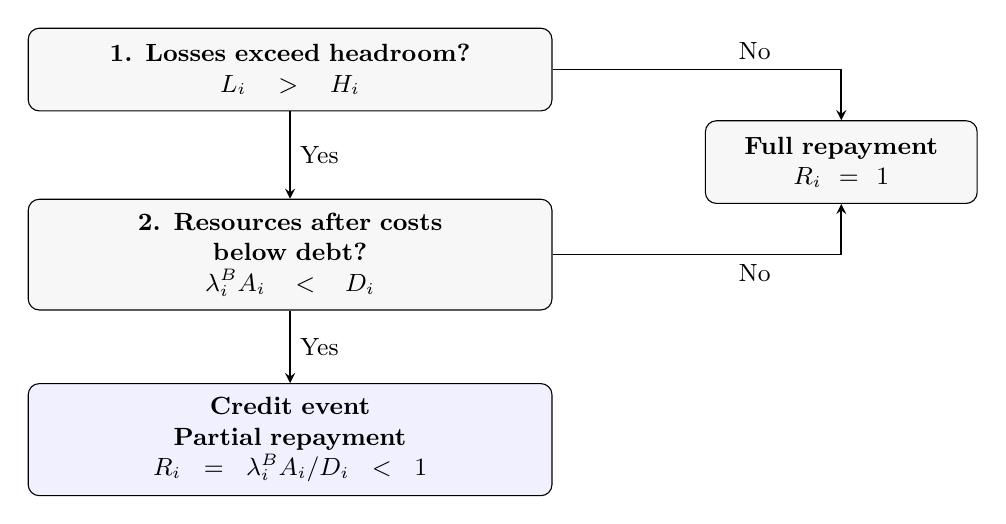
\begin{tikzpicture}[x=1cm,y=1cm,>=stealth,
 test/.style={draw,rounded corners,align=center,text width=6.3cm,minimum height=1.05cm,inner sep=5pt,fill=black!3,font=\small\linespread{1}\selectfont},
 outcome/.style={draw,rounded corners,align=center,text width=6.3cm,minimum height=1.05cm,inner sep=5pt,font=\small\linespread{1}\selectfont}]
 \node[test] (headroom) at (0,0) {\mbox{\textbf{1. Losses exceed headroom?}}\\$L_i>H_i$};
 \node[test] (shortfall) at (0,-2.35) {\textbf{2. Resources after costs}\\\textbf{below debt?}\\$\lambda_i^B A_i<D_i$};
 \node[outcome,fill=blue!6] (partial) at (0,-4.7) {\textbf{Credit event}\\\textbf{Partial repayment}\\$R_i=\lambda_i^B A_i/D_i<1$};
 \node[outcome,text width=3.1cm,fill=black!3] (full) at (7,-1.175) {\textbf{Full repayment}\\$R_i=1$};
 \draw[->,line width=.6pt] (headroom.south) -- node[right,font=\small]{Yes} (shortfall.north);
 \draw[->,line width=.6pt] (shortfall.south) -- node[right,font=\small]{Yes} (partial.north);
 \draw[->,line width=.6pt] (headroom.east) -| node[pos=.35,above,font=\small]{No} (full.north);
 \draw[->,line width=.6pt] (shortfall.east) -| node[pos=.35,below,font=\small]{No} (full.south);
\end{tikzpicture}

\end{figure}


\subsection{Equilibrium and the source of multiplicity}\label{subsec:recovery-wedge}

A banking equilibrium in state $s$ is a vector $\mathbf{R}$ satisfying \eqref{eq:bank_repayment} for every bank, using the receipts generated by that same vector. Write this fixed-point problem as $\mathbf{R}=F_s(\mathbf{R})$. The repayment map $F_s$ is nondecreasing: larger receipts from debtor banks cannot reduce a creditor bank's repayment. Since $F_s$ is nondecreasing and maps $\mathcal K$ into itself, Tarski's fixed-point theorem ensures that a least and a greatest equilibrium exist.\footnote{Under the order that compares repayment rates bank by bank, $\mathcal K=[0,1]^{|\mathcal B|}$ is a complete lattice: every subset has a supremum and an infimum in $\mathcal K$. A nondecreasing map from a complete lattice into itself has a least and a greatest fixed point \citep[Theorem~1]{Tarski1955}. Continuity is not required, so the result applies despite the discontinuities caused by default costs.} Let $\mathcal E_0(s)$ be the set of equilibria without intervention, and write $R_j^e(s)$ for bank $j$'s repayment in equilibrium $e\in\mathcal E_0(s)$. Denote the greatest repayment vector by $\bar{\mathbf{R}}(s)$ and its equilibrium by $e^*(s)$. We call this outcome preferred because it maximizes every bank's repayment, without claiming a welfare ranking. Thus $\bar R_j(s)=R_j^{e^*(s)}(s)$. We call defaults that persist in this greatest-repayment outcome fundamental defaults.

Without default costs ($\lambda_i^B=1$ for every bank), equation~\eqref{eq:bank_repayment} reduces to capped pro-rata repayment, $R_i=\min\{1,A_i/D_i\}$, as in \citet{EisenbergNoe2001}. Total payment is then $D_iR_i=\min\{D_i,A_i\}$: it is continuous in resources, and a one-euro reduction in resources reduces payment by at most one euro. If every bank also owes a positive share of its debt to nonbank creditors, only a fraction of this payment reduction reaches other banks. Together, these two properties make the clearing map a contraction in total payments and imply a unique equilibrium. Deposit funding supplies the outside-creditor condition in the calibration. Appendix~\ref{app:solver_details} gives the proof and relates this condition to Eisenberg and Noe's regularity assumption. The unique equilibrium can still contain bank defaults.

Allowing default costs ($\lambda_i^B<1$) preserves the outside-creditor condition and the monotonicity of the repayment map, but changes the payment rule. Crossing the distress threshold can now trigger a cost on the entire remaining estate: an arbitrarily small reduction in resources can cause a discrete drop in payment. This jump violates the bound on payment changes used in the contraction argument, so outside creditors alone no longer guarantee uniqueness. Continuity alone would not establish uniqueness either; the benchmark argument uses the quantitative bound together with payments to outside creditors. Lower counterparty payments can cause bank defaults even without default costs. The distinction here is that, with default costs, repayment feedback can sustain both a full-repayment equilibrium and an equilibrium with mutually reinforcing bank defaults, for the same exposures and nonbank resources. The following example illustrates this possibility.

\paragraph{A two-bank illustration}
Fix a sovereign state and consider two identical banks. Each owes one unit: half to the other bank and half to nonbank creditors. Each has fixed outside receipts of .51 and the same default-cost parameter $\lambda_i^B=\lambda$. With an accounting-insolvency threshold $T_i=D_i=1$, bank $i$'s assets and repayment are
\[
 A_i=.51+.5R_j,\qquad
 R_i=\begin{cases}1,&A_i\geq1,\\
 \lambda A_i,&A_i<1,\end{cases}\qquad i\ne j.
\]
Without default costs ($\lambda=1$), the unique equilibrium has both banks repaying fully: each receives $A_i=1.01$. With $\lambda=.90$, this equilibrium remains valid, but there is also an equilibrium in which both banks default. Their common repayment solves
\[
 R=.90(.51+.5R),\qquad
 R=\frac{.459}{.55}\simeq.835.
\]
Assets are then approximately .927, below the default threshold, so both defaults are consistent with the repayment rule. The share of debt owed to nonbank creditors remains 50\%: multiplicity arises because repayment jumps from a left limit of .90 to one when assets reach the threshold.

\subsection{Solution}

We solve the clearing system separately for every sovereign state. In each state, we enumerate all bank credit-event sets, solve for the candidate repayment vector associated with each set, and retain every vector that satisfies the original repayment rule. This procedure identifies all equilibria, including the least and greatest repayment vectors; Appendix~\ref{app:solver_details} gives the algorithm. State-by-state equilibria do not require probabilities for sovereign states. These probabilities enter only when computing averages across states.

To distinguish direct losses from repayment feedback, we also identify defaults under full interbank repayment: we apply the sovereign and private-credit losses while assuming that every interbank claim is paid in full, and check which banks breach their distress thresholds. These defaults are caused by direct losses alone. Comparing this diagnostic with equilibrium clearing shows how endogenous repayment shortfalls change bank outcomes. If no bank defaults in this diagnostic, full bank repayment is an equilibrium, but default costs may allow additional equilibria with lower repayments. The diagnostic is a benchmark calculation, not a sequence of settlements.

